\documentclass[a4paper,11pt]{article}

\usepackage{graphicx}
\usepackage{subfig,hyperref}
\newcommand{\HRule}{\rule{\linewidth}{0.5mm}}

\begin{document}
\pagenumbering{alph}
\begin{titlepage}
\begin{center}

\textsc{\LARGE CMSC726 Machine Learning}\\[1.5cm]

\textsc{\Large Project 3}\\[0.5cm]

\HRule \\[0.5cm]

{ \huge \bfseries Unsupervised Learning}\\[0.4cm]

\HRule \\[1.5cm]

{\large Angjoo Kanazawa, Ran Liu, and Austin Myers}

\vfill

{\large December 6, 2011}

\end{center}
\end{titlepage}
\pagenumbering{arabic}

\section{PCA and Kernel PCA}
\subsection{WU1}
\textsf{Depending exactly on your random data, one or more of these lines might
not pass exactly through the data as we would like it to. Why not?}\vspace{0.1in}

As shown in figure \ref{figures:WU1}, the eigenvectors are actually what we would
expect, with the first vector accounting for the axis of skew and the second vector
orthogonal to the first. This is intuitive since the skew should be the primary
source of variance, and the second eigenvector should simply be perpendicular
to the first since it's a two dimensional projected space.

\begin{figure}[!ht]
  \begin{center}
  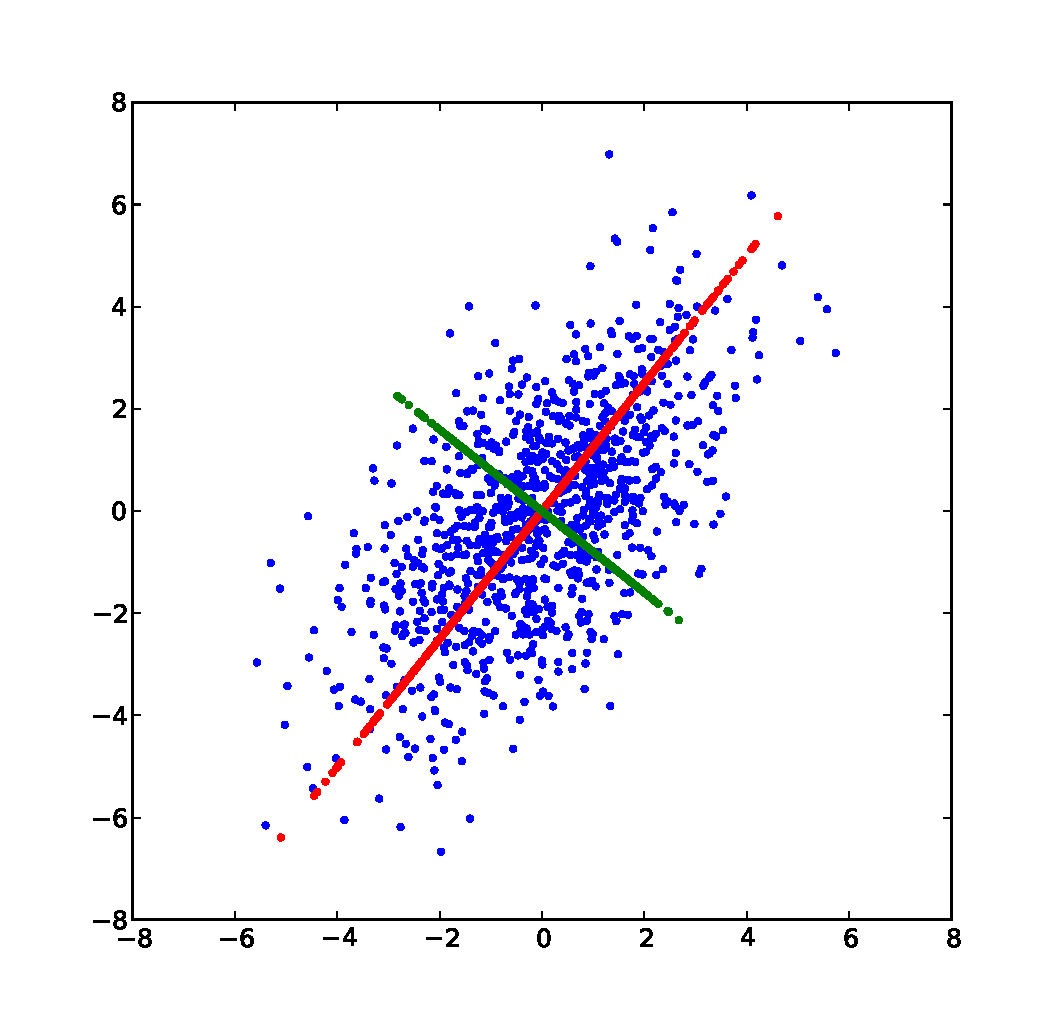
\includegraphics[width=4in]{WU1.pdf}
  \caption{Eigenvectors and projected data}
  \label{figures:WU1}
  \end{center}
\end{figure}

\subsection{WU2}
\textsf{Plot the normalized eigenvalues (include the plot in your writeup). 
How many eigenvectors do you have to include before you've accounted 
for 90\% of the variance? 95\%? (Hint: see function cumsum.)}\vspace{0.1in}

We need to include 81 eigenvectors to account for 90\% of the variance and
135 eigenvectors to account for 95\%. The eigenvalues are shown in figure
\ref{figures:WU2a} and the cumulative sum of the eigenvalues is shown in
figure \ref{figures:WU2b} with labels for the two points of interest.

\begin{figure}[!ht]
  \begin{center}
  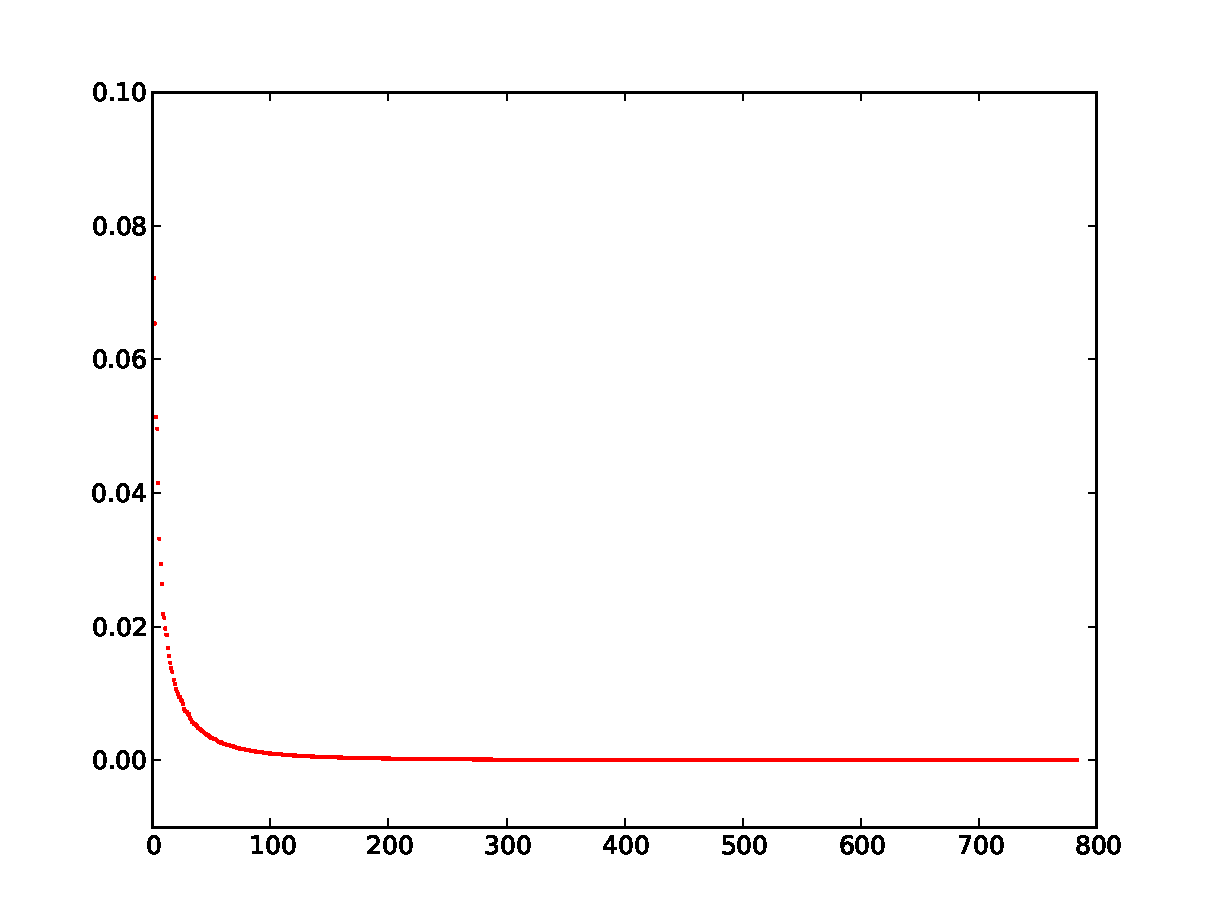
\includegraphics[width=4in]{WU2_a.pdf}
  \caption{Plot of the normalized eigenvalues}
  \label{figures:WU2a}
  \end{center}
\end{figure}

\begin{figure}[!ht]
  \begin{center}
  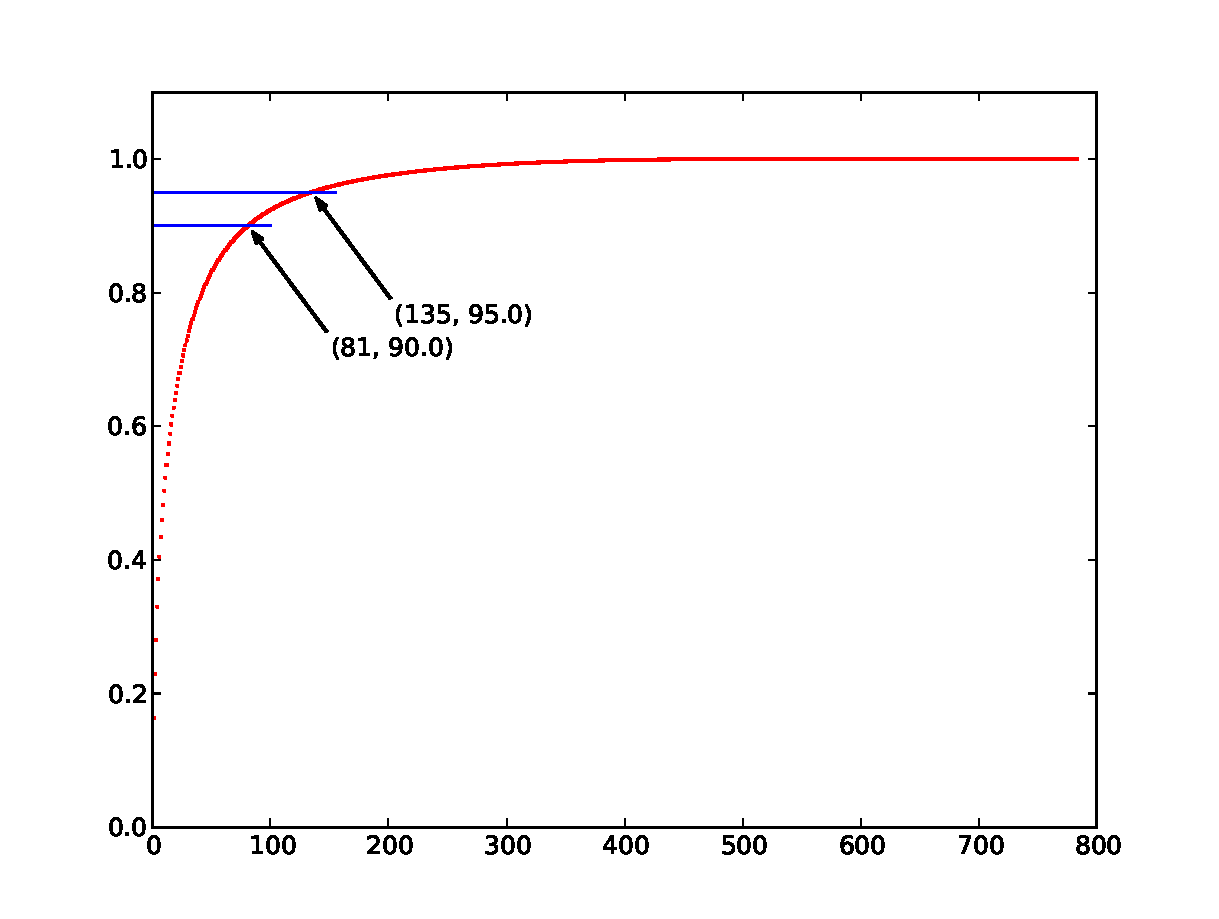
\includegraphics[width=4in]{WU2_b.pdf}
  \caption{Plot of the normalized eigenvalues}
  \label{figures:WU2b}
  \end{center}
\end{figure}

\subsection{WU3}
\textsf{Do these look like digits? Should they? Why or why not?
(Include the plot in your write-up.)}\vspace{0.1in}

Although most of the images in figure \ref{figures:WU3a} do not look
like digits, a few do resemble simple primitives which some digits
share. These eigenvectors likely contribute significantly to the basic
structure of some digits, but most of the eigenvectors are encoding
detail information which is not easily recognizable. We can show how
only a few eignevectors encode some basic structure by taking the 
eigenvectors and the projected data and trying to reconstruct the original dataset.
With 784 eigenvectors, the reconstructed data appears to be very accurate 
as shown in \ref{figures:WU3b}, but with only 5 we still see that some simple
structures have been captured as shown in \ref{figures:WU3c} which shows why
some of the eignvectors in figure \ref{figures:WU3a} may look like simple digit structures.

\begin{figure}[!ht]
  \begin{center}
  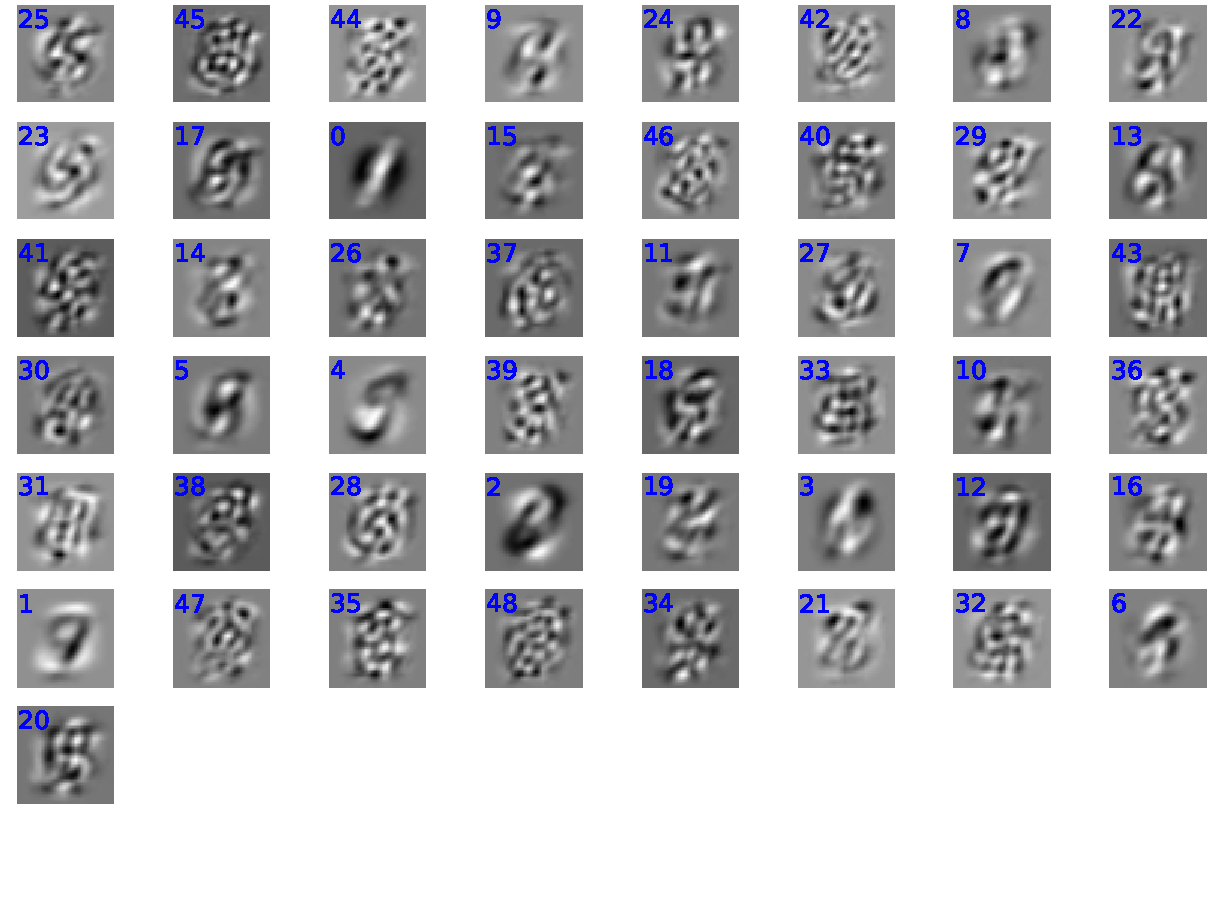
\includegraphics[width=4.5in]{WU3_a.pdf}
  \caption{Plot of eigenvectors using vanilla pca}
  \label{figures:WU3a}
  \end{center}
\end{figure}

\begin{figure}[!ht]
  \begin{center}
  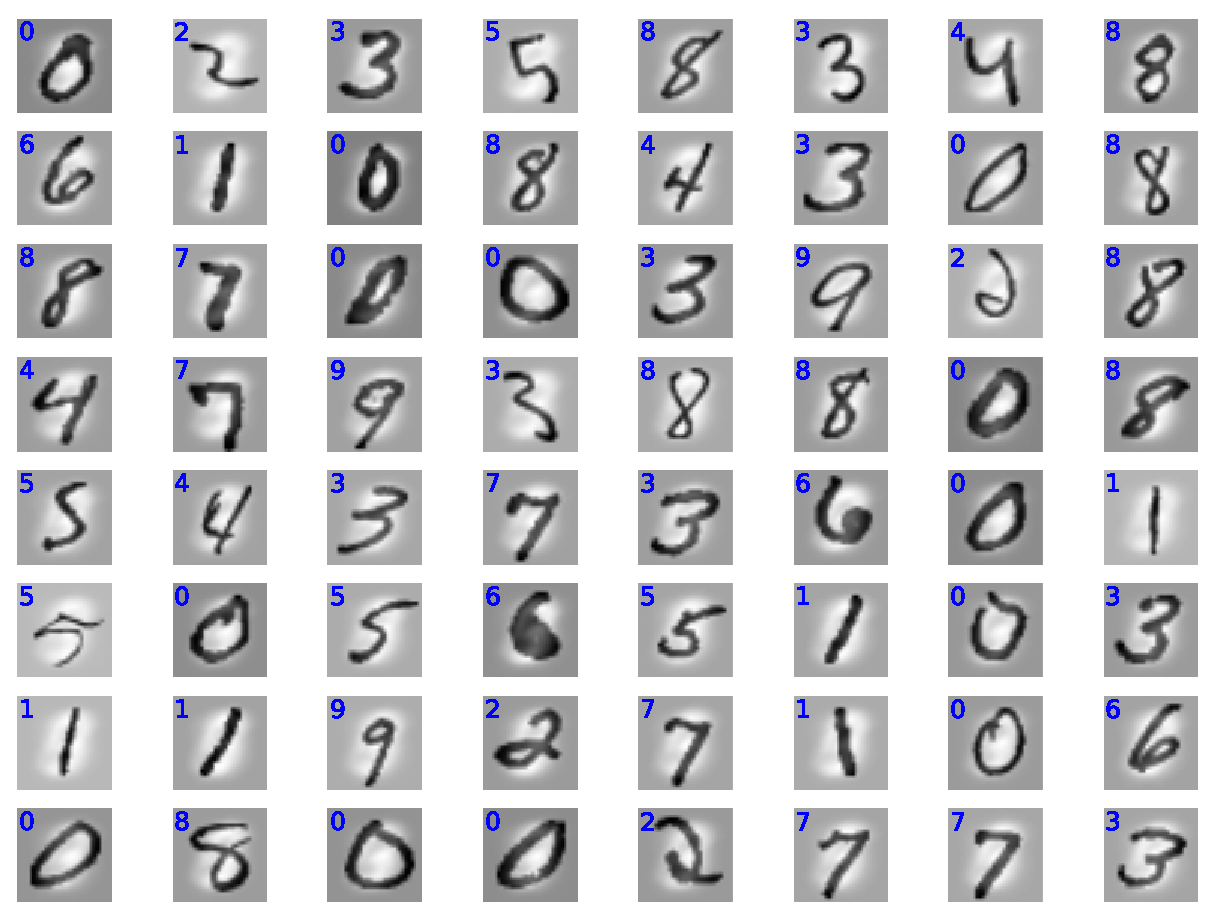
\includegraphics[width=4.5in]{WU3_b.pdf}
  \caption{Reconstructed digit images using 784 eigenvectors}
  \label{figures:WU3b}
  \end{center}
\end{figure}

\begin{figure}[!ht]
  \begin{center}
  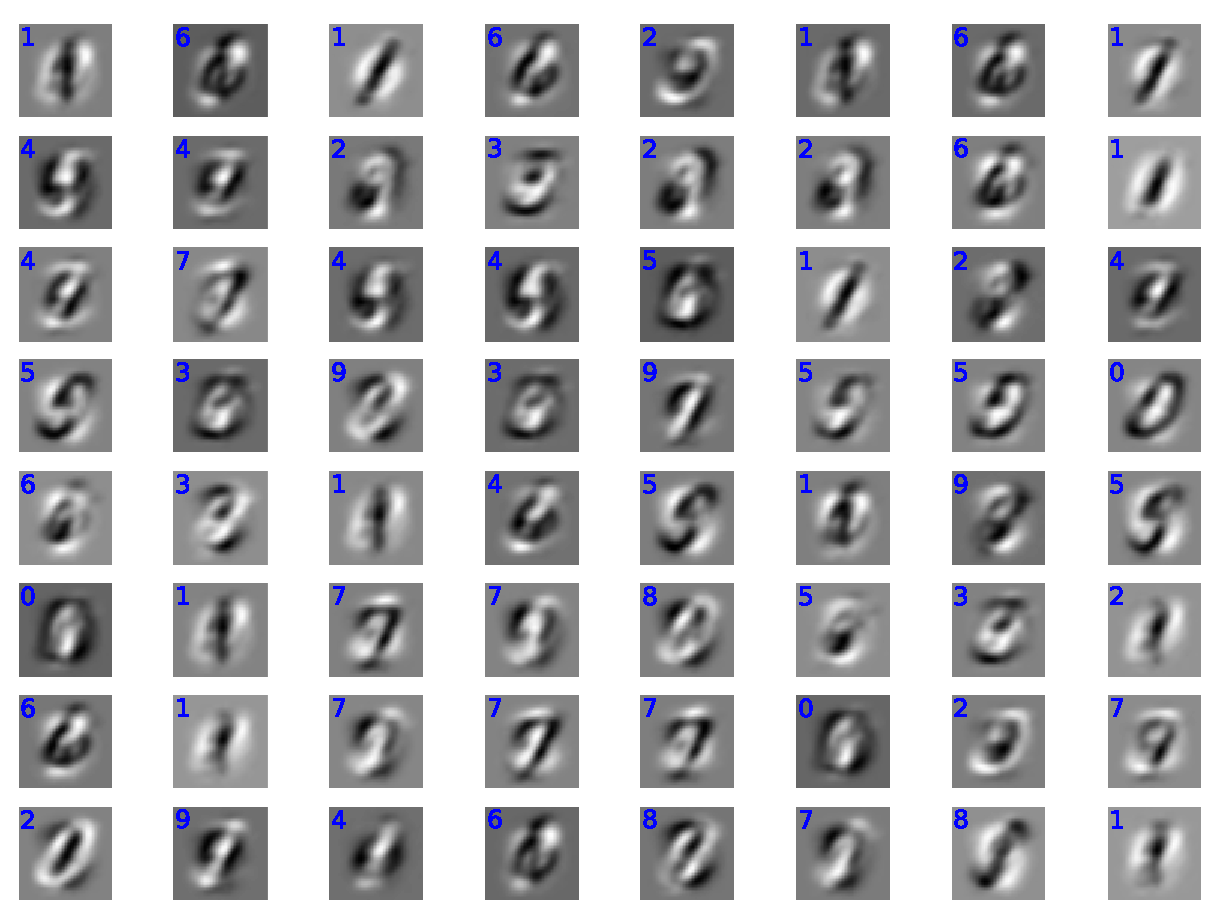
\includegraphics[width=4.5in]{WU3_c.pdf}
  \caption{Reconstructed digit images using only 5 eigenvectors}
  \label{figures:WU3c}
  \end{center}
\end{figure}

\pagebreak
\subsection{WU4}
\textsf{Why does vanilla PCA find this data difficult? What is the
significance of the relatively large value of the eigenvalues
here?}\vspace{0.1in}

PCA tries to find patterns in dataset that highlights the differences
and similarities. Once we find such patterns, we can reduce the
dimensionality of the data without losing too much
information. Vanilla PCA will find this data difficult to characterize
because the circular distribution of points cannot be represented
using only two eigenvectors in two dimensions since this corresponds to 
linear combinations. Consequently, both of the eigenvalues are relatively similar because
there is no one direction that maximizes the variance.

\subsection{WU5}
\textsf{Did PCA do what we might want it to? Why or why not? Include
the plot to justify your answer.}\vspace{0.1in}

PCA did not do what we might want it to since we want the projected
red data and the blue data points to be easily seperable or clustered.
As shown in figure \ref{figures:WU5} the data has not been separated.
Following from WU4, PCA does not work well because the circular distribution 
of points cannot be represented using linear combinations of two dimensional vectors.

\begin{figure}[!ht]
  \begin{center}
  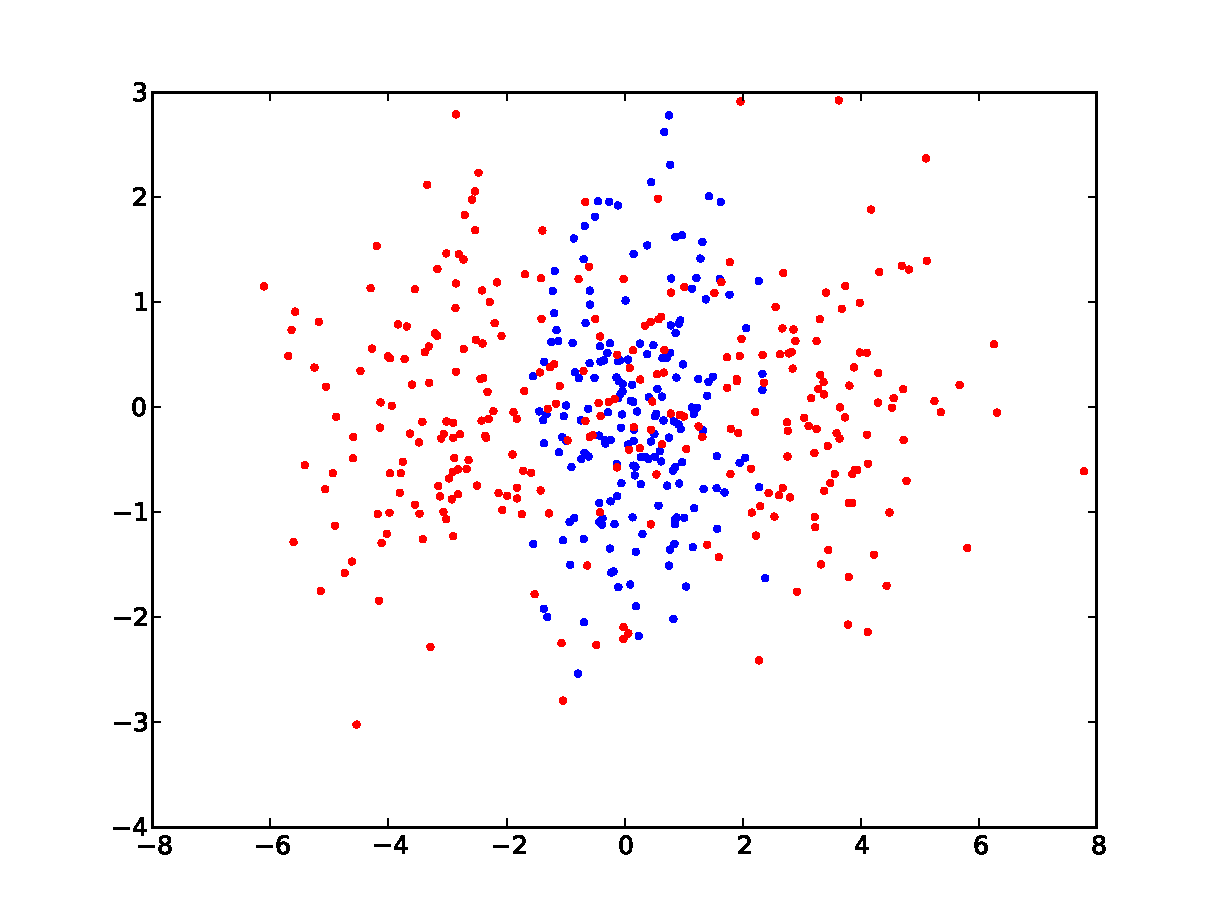
\includegraphics[width=4.5in]{WU5.pdf}
  \caption{Projected data using eigenvectors found by vanilla PCA}
  \label{figures:WU5}
  \end{center}
\end{figure}

\subsection{WU6}
\textsf{How do the eigenvalues here compare to the linear case? What
does this tell you? How does the plot look? How might this be useful
for supervised learning?}\vspace{0.1in}

Compared to the linear case, the eigenvalues are much smaller in
magnitude $(0.08121919,  0.05313867)$, and the ratio of the first
eigenvalue to the second eigenvalue is around 1.5, where the
linear case exhibited a ratio that was closer to 1. 
This means that KPCA using rbf1 managed to...

As shown in figure \ref{figures:WU6}, the projection clusters 
red datapoints into a small space, whereas blue datapoints a 
left dispersed but seperate from the red points by a small margin.
This is useful for supervised learning because we can use KPCA
projection to cluster the training data points that belong in 
the same class as much as possible, and feed that projected data to the classifier.
Since we have the labels we can try different kernels and use the one
that gives us the largest margin and is the easiest for our classifier to learn.

\begin{figure}[!ht]
  \begin{center}
  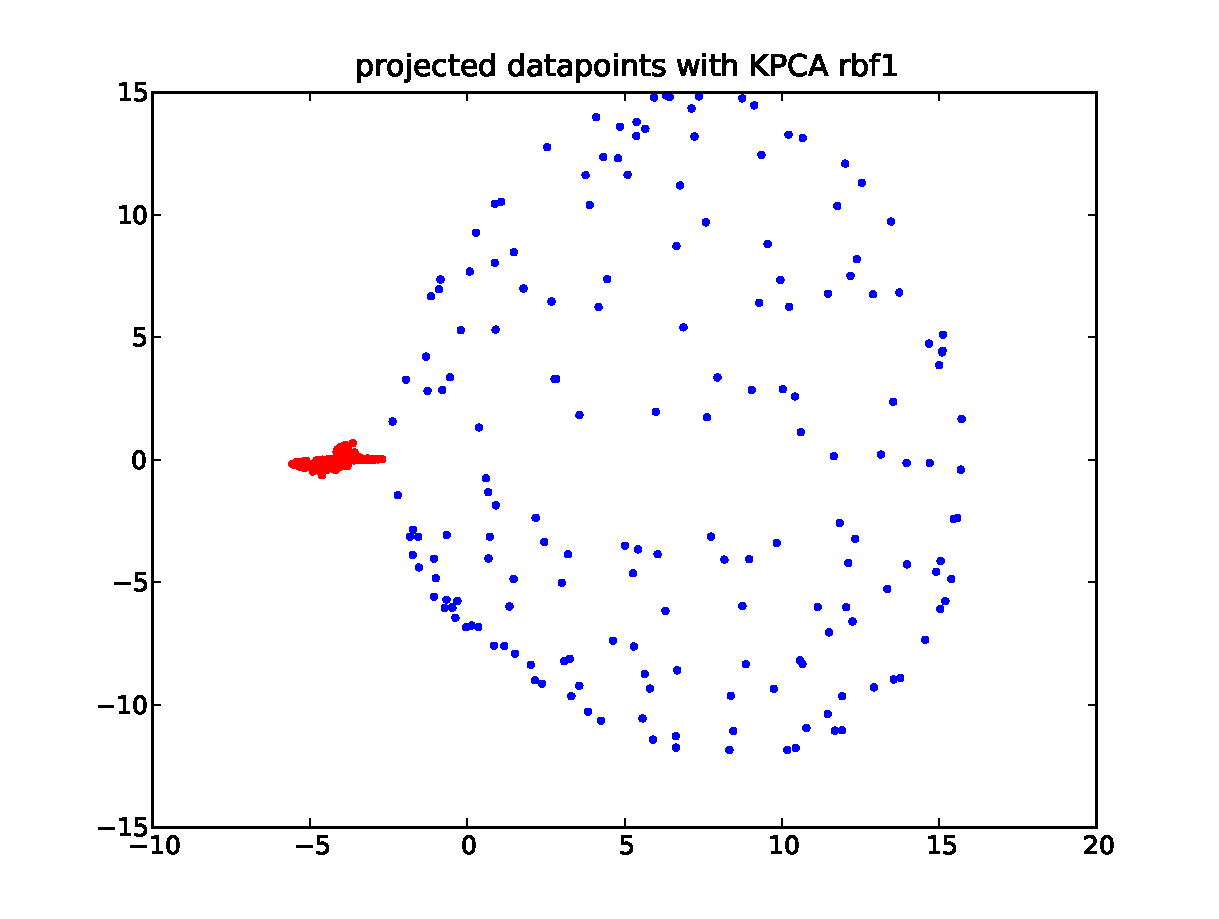
\includegraphics[width=4.5in]{WU6.pdf}
  \caption{Projected data using KPCA and rbf1}
  \label{figures:WU6}
  \end{center}
\end{figure}

\pagebreak
\subsection{WU7}
\textsf{Experiment with different kernels, and perhaps interpolations 
of different kernels. Try to find a kernel that gets as much of the 
variance on the first two principle components as possible. Report your 
kernel and a plot of the data projected into 2d under that kernel.}\vspace{0.1in}

The standalone kernel that seemed to perform the best were rbf0\_2 and rbf0\_5,
as shown in figure \ref{figures:WU7_rbf0_2} and figure \ref{figures:WU7_rbf0_5}
respectively. The former seemed to nicely separate the red and blue points,
and the latter seemed to cluster the red points, so we tried to combine the two 
kernels multiplicatively. The result, shown in figure \ref{figures:WU7_combo},
was actually not much different than rbf0\_5, but it seemed to be the best using 
combinations of the standard kernel functions. Finally, we tried to make our own
function based on our knowledge of the data, yielding the function and result in
figure \ref{figures:WU7_final}. This function has reduced all the red data and blue
data to separate points, however the function is probably not positive semi-definite,
though this assertion has not been verified. Regardless, these are interesting
examples of kernel function that might be useful if this type of data needed to be classified.

\begin{figure}[!ht]
  \centering
  \subfloat[rbf0\_2]{\label{figures:WU7_rbf0_2}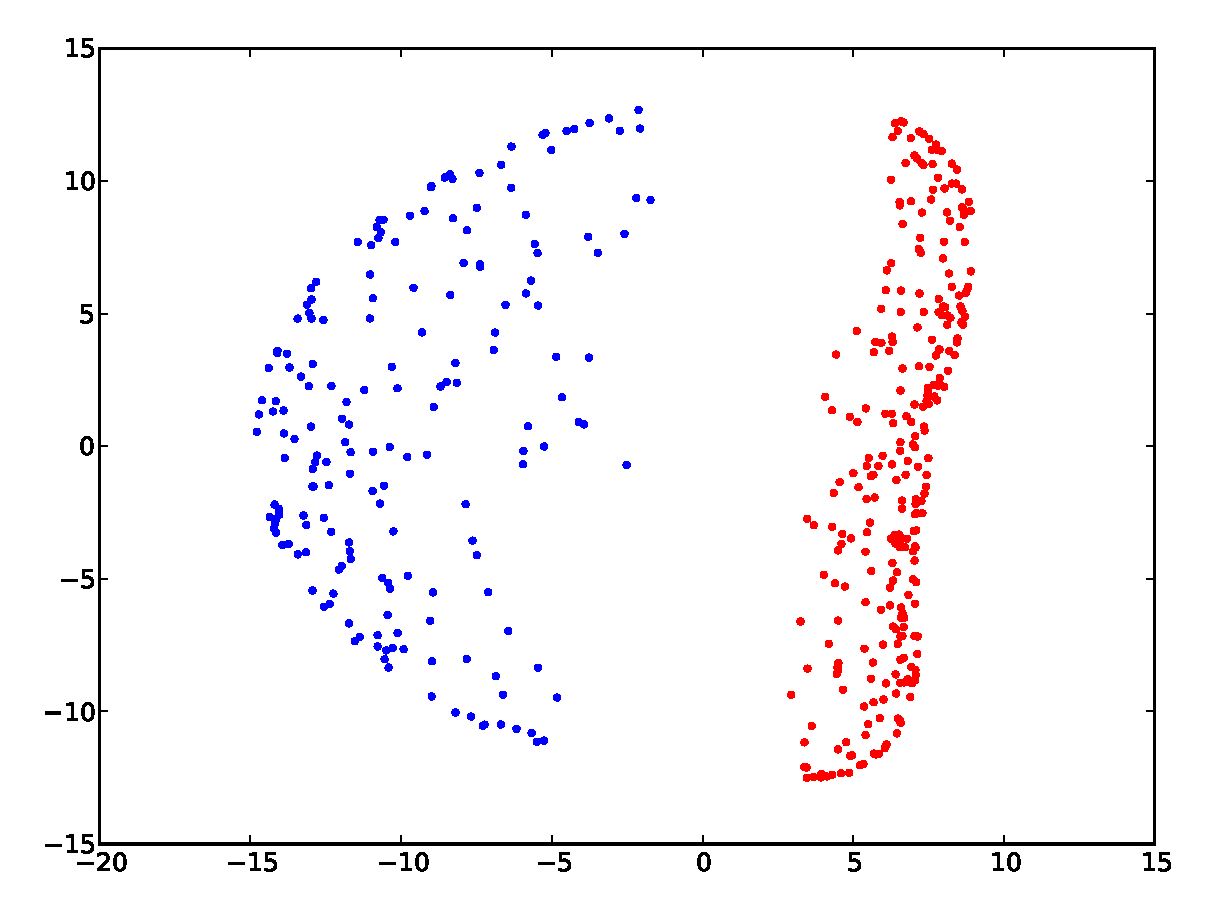
\includegraphics[width=2.25in]{WU7_rbf_0_2.pdf}}
  \subfloat[rbf0\_5]{\label{figures:WU7_rbf0_5}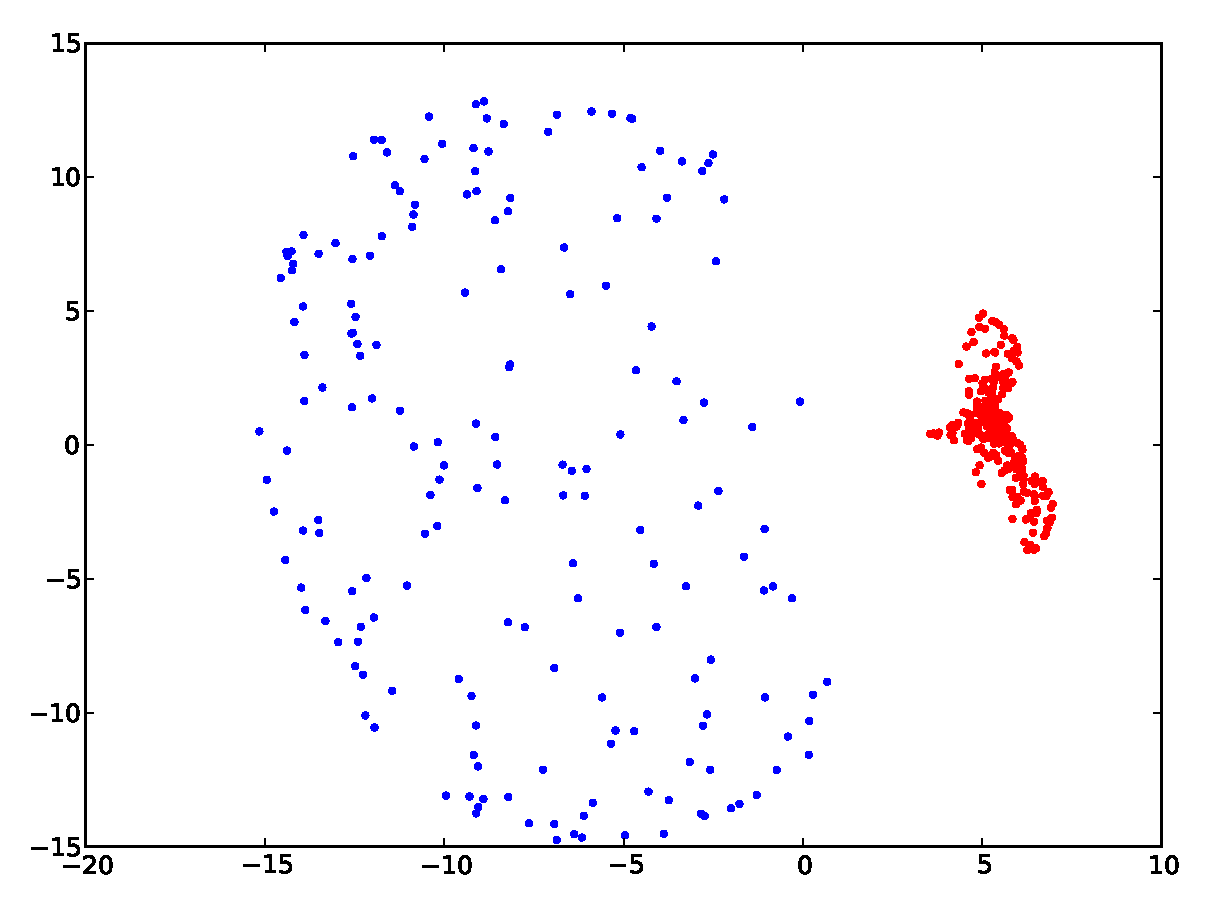
\includegraphics[width=2.25in]{WU7_rbf_0_5.pdf}}  
  \caption{Projected data using KPCA and standard kernels}
\end{figure}

\newpage

\begin{figure}[!ht]
  \begin{center}
  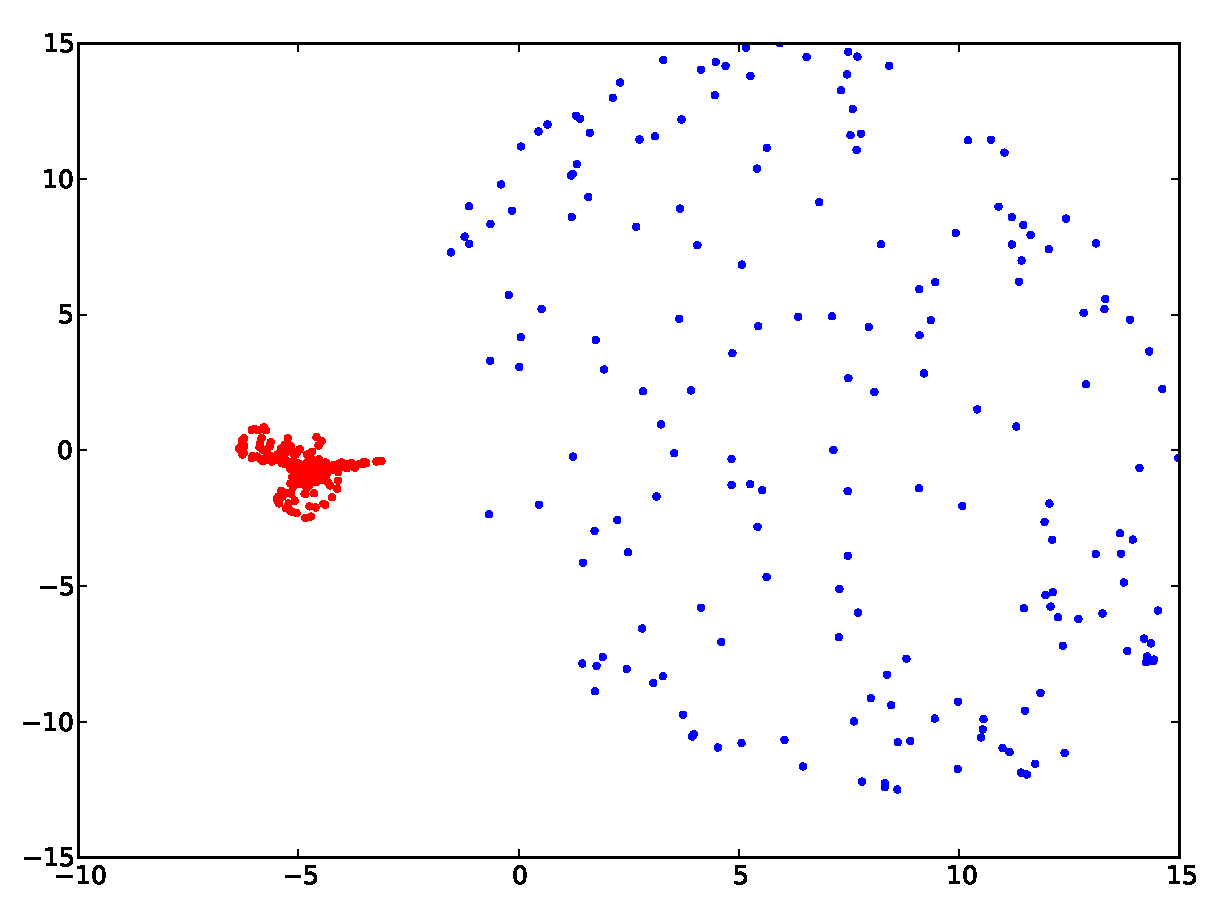
\includegraphics[width=4in]{WU7_combo.pdf}
  \caption{Projected data using KPCA and rbf0\_2 and rbf0\_5 combined}
  \label{figures:WU7_combo}
  \end{center}
\end{figure}

\begin{figure}[!ht]
  \begin{center}
  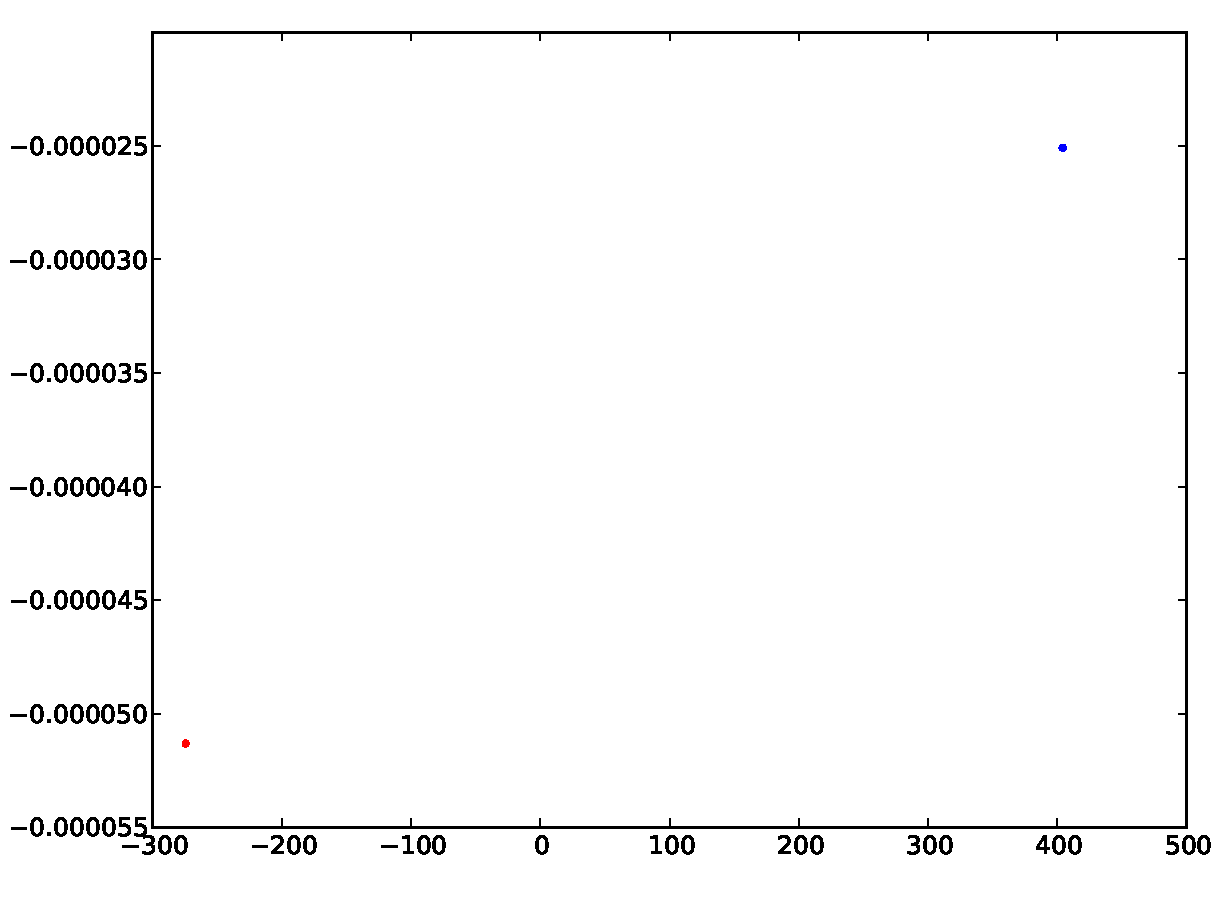
\includegraphics[width=4in]{WU7_final.pdf}
  \caption{Projected data using KPCA and the custom function}
  \[\frac{1000}{1 + e^{-1000 \sqrt{(x \cdot x) - 2.75}} + e^{-1000 \sqrt{(z \cdot z) - 2.75}}}\] 
  \label{figures:WU7_final}
  \end{center}
\end{figure}

\newpage
\section{HMMs:Viterbi}
\subsection{WU8}
\textsf{Find two different observation sequences of length four that
differ only in one place, but differ in more than one place in the
guessed output.}\vspace{0.1in}

%hmm.viterbi(array([0,1,1,1]), a, b, pi) # 0 0 0 0
%hmm.viterbi(array([0,1,2,1]), a, b, pi) # 0 0 1 1

One example of this effect can be found with observation sequences
[0,1,1,1] and [0,1,2,1] which differ only in the third observed emission,
but which yield predictions of [0,0,0,0] and [0,0,1,1] respectively.
Thus, the predictions differ in two states where the observations only
differ in one.

\section{HMMs:Forward-backward}
\subsection{WU9}
\textsf{Why does EM settle in this configuration? What is it saying? 
What happens when you use three states instead of two? 
What's the resulting probability of the data? 
What about four states? What happens and why?}\vspace{0.1in}

EM settles in this configuration because it has found a local minima. The
$\hat \pi = [1,0,0]$ means that we always start at state 0. We also get $P(X_t=0|X_{t-1}=0)= 0$,
i.e. when we transition we always go to a different state. All
together the results say that the most likely state sequence is the
one where states alternate every step.

If we use three states instead of two, similar behavior happens with
$\hat \pi$. One state has a probability of 1 and the rest gets 0. But
in the transition probability, we do get a single state that
has positive probabilities for more than one states.

When we increase the states to four, the behavior is still similar in
a way that we have very high probabilities for specific transitions
and emissions, but the probability of transition is more distributed.

This is because the way we produce the intial HMM is random. When
there are only two states, the only way for the final probabilities to
be well distributed is if initial transition from state 0 to state 0
and state 0 to state 1 is close i.e. 1/2, 1/2. If anything, it's very
easy for EM to exaggerate the probability of the bigger one.

But as the number of states increases, the likelihood of uniformly
distributin the initial HMM probabilities increases. So we get more
reasonable (unskewed) results for EM.

\pagebreak
\subsection{WU10}
\textsf{Run EM on this data using two states. 
Run it a few times until you get a final log probability at least -9250. 
(It should happen in two or three trials. This will take a few minutes to run.) 
When you do this, it will print out the resulting initial state probabilities, 
transition probabilities and emission probabilities. 
What has it learned? Include all of this output in your
write-up.}\vspace{0.1in}

It has learned the probability of spaces and vowels vs the probability
of consonants! State 0 emits all spaces or vowels and state 1 emits
consonants. It also makes sense that the transition from state 0 to
state 0 is lower than that of state 1, because it's more likely that
consonants are followed by consonants than that vowels are followed by vowels.

The output of EM om this data is:
\begin{verbatim}
Initial state probabilities:
	state(0):	7.4252e-202
	state(1):	1

Transition probabilities:
FROM\TO
	0 	1 
0 	0.245207 	0.754793 
1 	0.720637 	0.279363 

Emission probabilities:
	State 0:
		_  0.362509
		e  0.232741
		a  0.125778
		o  0.120613
		i  0.104855
		u  0.04369
		y  0.00345083
		t  0.00258696
		k  0.0019353
		q  0.00121219
		g  0.000467752
		s  0.000115461
		c  2.34141e-05
		p  1.62641e-05
		l  3.6812e-06
		d  1.16317e-06
		b  1.69503e-07
		h  1.26829e-08
		w  8.21573e-12
		r  1.47438e-14
		f  5.26943e-15
		m  4.67596e-15
		j  2.11457e-16
		n  2.45545e-17
		x  4.24731e-29
		v  3.78819e-34
		z  3.08129e-51
	State 1:
		t  0.141537
		r  0.102944
		n  0.0971604
		s  0.0970502
		h  0.094847
		d  0.0670858
		l  0.0636134
		c  0.0479795
		m  0.0439535
		f  0.0347001
		y  0.0337207
		p  0.0329496
		w  0.0306518
		b  0.0260249
		g  0.0244221
		v  0.0202417
		k  0.0166601
		_  0.0155547
		a  0.00316851
		x  0.00173501
		j  0.00173501
		u  0.00168636
		z  0.000578336
		o  2.52571e-07
		e  6.20806e-09
		i  2.8181e-11
		q  1.18265e-17
\end{verbatim}
\end{document}
